\documentclass[12pt,a4paper,oneside,titlepage,liststotoc,bibtotoc]{scrreprt}
\usepackage[utf8]{inputenc}
\usepackage[top=2.5cm,bottom=2.5cm,left=2.5cm,right=2.5cm,includehead,includefoot]{geometry}
\usepackage[ngerman]{babel}
\usepackage{graphicx}
\usepackage{hyperref}
\usepackage{setspace}
\usepackage{fancyhdr}
\usepackage{acronym}
\usepackage{listings}
\usepackage{float}

% Infos
\newcommand{\titel}{Projektbericht}
\newcommand{\untertitel}{Scoreboard}
\newcommand{\studiengang}{Informatik}
\newcommand{\studienrichtung}{Angewandte Informatik}
\newcommand{\autorone}{Fabian Blatz}
\newcommand{\autortwo}{Sven Baumann}
\newcommand{\autorthree}{Marcel Bohrmann}
\newcommand{\autorfour}{Christian Gutermann}
\newcommand{\kurs}{TINF15B4}
\newcommand{\abgabe}{3. Oktober 2017}
\newcommand{\betreuerdhbw}{Prof. Dr. Ralph Lausen}
\newcommand{\jahr}{2018}

% Logos
\newcommand{\logodhbw}{
\includegraphics[width=6cm]{img/logos/dhbw}}

% Abkürzungen
\newcommand{\ua}{\mbox{u.\,a.\ }}
\newcommand{\zb}{\mbox{z.\,B.\ }}
\newcommand{\heisst}{\mbox{d.\,h.\ }}
\newcommand{\bs}{$\backslash$}

% Definition der Kopf- und Fußzeilen
\fancyhf{}
\fancyhead[R]{\sffamily \nouppercase{\leftmark}}
\fancyfoot[C]{\sffamily \thepage}
%\renewcommand{\chapterpagestyle}{scrheadings}

\pagestyle{fancy}
\onehalfspacing

\begin{document}

\begin{titlepage}
\sffamily

% Logos
\logodhbw \hfill \\[1ex]

\begin{center}

% Text
\huge{\textsc{\textbf{\titel}}}\\
\Large{\textbf{\untertitel}}\\[3ex]


\normalsize{Für die Vorlesung\\ Systemnahe Programmierung I \\[4ex]}

\Large{Studiengang \studiengang}\\
\normalsize{Studienrichtung \studienrichtung}\\
\normalsize{Duale Hochschule Baden-Württemberg Karlsruhe}\\[2ex]

Von\\
\autorone,\\
\autortwo,\\
\autorthree,\\
\autorfour \\[4ex]

% Tabelle
\begin{tabular}{ll}
Abgabedatum:					& \quad \abgabe\\
Kurs:                           & \quad \kurs\\ 
Dozent:	 						& \quad \betreuerdhbw\\ 
\end{tabular}
    
\end{center}

\end{titlepage}

\tableofcontents

\chapter{Einleitung}

\section{Motivation}

\section{Aufgabenstellung}

\chapter{Grundlagen}

\section{Assembler}

\section{Der 8051 Mikrocomputer}

\section{Entwicklungsumgebung MCU-8051 IDE}

\chapter{Konzept}
Die Nachfolgende Betrachtung dient der Analyse der benoetigten Module die zur korrekten Implementierung und Ausfuerhung des geplanten Scoreboards benoetigt werden.\\

\section{Analyse}
Zur vollstaendigen und korrekten Implementierung des geplanten Funktionsumpfangs sind folgende Komponenten von Noeten:
\begin{itemize}
	\item Anzeigemoeglichkeiten
	\item Speichermoeglichkeiten fuer den momentanen Spielstand
	\item Taster, um den Speicherstand zu inkrementieren, dekrementieren oder zurueckzusetzen
	\item Ein Konzept, um die Tasterbedienung moeglichst bedienerfreundlich zu gestalten
\end{itemize}

\subsection{Anzeige}
Fuer die Anzeige wurde ein Multiplex-LED-Display verwendet, welches folgende Eigenschaften aufweist:
\begin{itemize}
	\item 4x7 LED-Felder
	\item Gesteuert ueber 12-Pins an 2 Ports, in diesem Fall P2 und P3
\end{itemize}

\subsection{Speicherstruktur}
Die Speicherung des Spielstandes erfolgt in Port 1. Hierbei besitzt jeder Spieler 4 Bit, in denen Informationen zu seinem Punktstatus gespeichert werden können. Initialisert wird der Punktespeicher für jeden Spieler mit 0001. Wird dem Spieler ein Punkt gutgeschrieben so wird sein Teil des Port 1 auf 0011 gesetzt, sein Register wird auf den entsprechenden Wert von 15 gesetzt. Da für jeden Spieler die Zustände 0, 15, 30, 40 gespeichert werden müssen, genügt diese Codierung der Abbildung des Tennisspiels. 

\subsection{Taster}
Um das Scoreboard anzusteuern stehen dem Nutzer 3 Taster zur verfuegung, welche einem Punkt fuer den linken Spieler, dem rechten Spieler und einer Reset-Taste entsprechen. Da in der Simulationsumgebung leider keine Druckknoepfe sondern nur Schalter gibt, muss der Nutzer hier den Schalter eigenstaendig Ein- und wieder Ausschalten.

\subsection{Tasterroutine}
Da es nicht vom Nutzer erwartet werde kann, dass er es schafft, Taktgenau zwischen einzelnen Ueberpruefungen des Tasterstatus die Taste zu betaetigen, wurde eine Routine implementiert, um bei laengerer Tasterbetaetigung keine Mehrfachzaehlungen zu beguenstigen.

\section{Programmentwurf}
Für die Planung des Programms haben wir uns dse sogenannte Nassi-Schneidermann Diagramms bedient. Dies brachte den Vorteil mit sich, dass der Programmentwurf einfach in Assembler umzusetzen war. Hierzu verwendeten wir eine Methodenschreibweise welche eher in objektorientierten Sprachen verwendet wird, um eine bessere Lesbarkeit zu sichern.
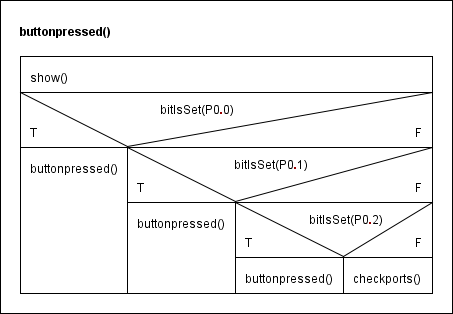
\includegraphics{img/buttonpressed}
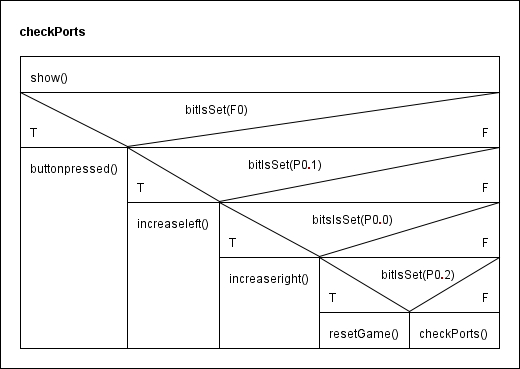
\includegraphics{img/checkPorts}
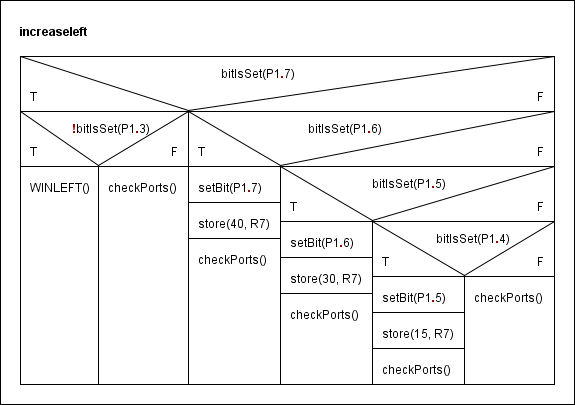
\includegraphics{img/increaseleft}
Für die Punktevergabelogik haben wir nun den Entwurf von increaseleft angefertigt, da sich für die Implementierung von increaseright nur die Bits innerhalb des Ports geändert haben. 
\chapter{Implementation}


\chapter{Zusammenfassung}




\begin{appendix}

\bibliographystyle{unsrt}
\raggedright
\bibliography{references/bibliothek}

\listoffigures
%\listoftables

	\chapter*{Abkürzungsverzeichnis}
\addcontentsline{toc}{chapter}{Abkürzungsverzeichnis}

\begin{acronym}[XML-RPC]

    \acro{BSP}{Beispiel}
    
\end{acronym}
    
\end{appendix}
	
\end{document}